\section{光的色散}\label{sec:1-9}

取一个棱镜,照图 \ref{fig:1-33} 那样,让一束白光(例如太阳光)穿过狭缝射在棱镜上。
可以看到,白光通过棱镜以后不但改变了方向,而且在白纸屏上形成一条彩色的光带。
\begin{figure}[htbp]
    \centering
    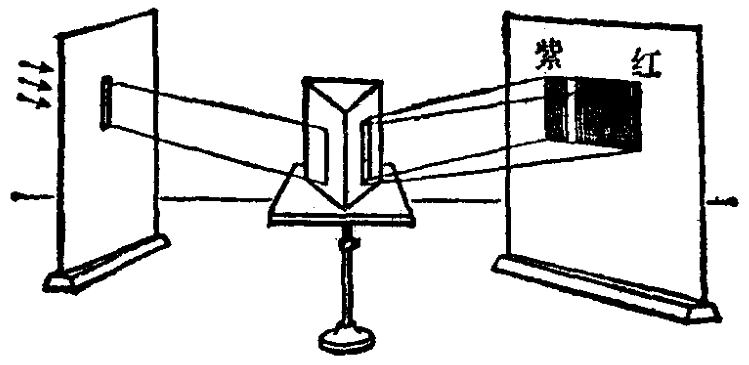
\includegraphics[width=0.6\textwidth]{../pic/czwl2-ch1-33}
    \caption{白光的色散}\label{fig:1-33}
\end{figure}
这条彩色光带上的颜色,从一端到另一端依次是红、橙、黄、绿、蓝、靛、紫。
这表明白光通过棱镜以后分解成各种色光。

\begin{figure}[htbp]
    \centering
    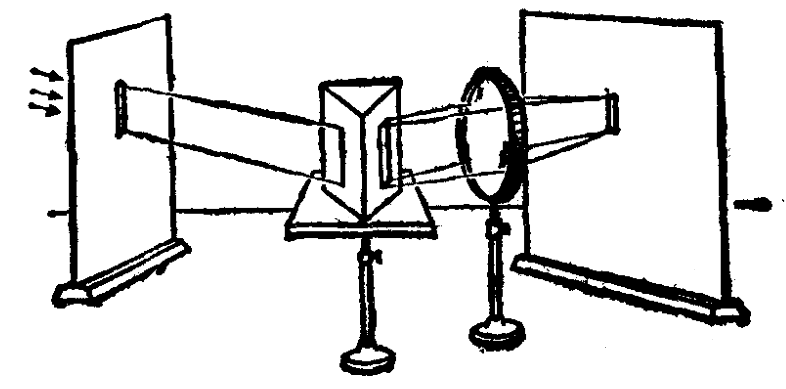
\includegraphics[width=0.6\textwidth]{../pic/czwl2-ch1-34}
    \caption{}\label{fig:1-34}
\end{figure}

如果照图 \ref{fig:1-34} 那样,把一个凸透镜放在棱镜和白纸屏之间,使这些色光会聚在纸屏上,
纸屏上就会出现一条白色光带。这表明色光合在一起又成了白色。

在图 \ref{fig:1-33} 的实验里,假如在纸屏上开一条狭缝,使彩色光带中的某种色光通过它,
再射到第二个棱镜上,那么这种色光通过第二个棱镜以后,就只改变方向,而不再分解成其他的色光了。

从上面的实验知道,白光是由各种色光混合而成的,白光通过棱镜以后,
分解成的各种色光是具有单纯颜色的光,不能再分解成其他的色光。

不能再分解的色光叫做\textbf{单色光},
由单色光混合成的光叫做\textbf{复色光}。
复色光分解成单色光的现象,叫做光的\textbf{色散}。


